% Pengaturan ukuran teks dan bentuk halaman dua sisi
\documentclass[10pt,twoside]{report}

% Pengaturan ukuran halaman dan margin
\usepackage[a5paper,top=25mm,left=25mm,right=20mm,bottom=25mm]{geometry}

% Pengaturan ukuran spasi
\usepackage[singlespacing]{setspace}

% Judul dokumen
\title{Buku Laporan Kerja Praktik ITS}
\author{Wahid, Yusuf Nur \and Priyanto, Helmika Mahendra}

% Pengaturan format bahasa
\usepackage[indonesian]{babel}

% Pengaturan detail pada file PDF
\usepackage[pdfauthor={\@author},bookmarksnumbered,pdfborder={0 0 0}]{hyperref}

% Pengaturan jenis karakter
\usepackage[utf8]{inputenc}

% Pengaturan ukuran indentasi paragraf
\setlength{\parindent}{2em}

% Pengaturan ukuran spasi paragraf
\setlength{\parskip}{0.5ex}

% Package lainnya
\usepackage{etoolbox} % Mengubah fungsi default
\usepackage{enumitem} % Pembuatan list
\usepackage{lipsum} % Pembuatan template kalimat
\usepackage{graphicx} % Input gambar
\usepackage{longtable} % Pembuatan tabel
\usepackage[table,xcdraw]{xcolor} % Pewarnaan tabel
\usepackage[numbers]{natbib} % Kutipan artikel
\usepackage{eso-pic} % Pembuatan background
\usepackage{changepage} % Pembuatan teks kolom
\usepackage{wrapfig} % Wrapping gambar
\usepackage{comment} % Long comment
\usepackage{tabto} % \tab command

% Definisi untuk "Hati ini sengaja dikosongkan"
\def\kosong{
  \vspace*{\fill}
  \begin{center}\textit{Halaman ini sengaja dikosongkan}\end{center}
  \vfill
}
\patchcmd{\cleardoublepage}{\hbox{}}{\kosong}{}{}

% Pengaturan penomoran halaman
\usepackage{fancyhdr}
\fancyhf{}
\renewcommand{\headrulewidth}{0pt}
\pagestyle{fancy}
\fancyfoot[CE,CO]{\thepage}
\patchcmd{\chapter}{plain}{fancy}{}{}
\patchcmd{\chapter}{empty}{plain}{}{}

% Pengaturan format judul bab
\usepackage{titlesec}
\titleformat{\chapter}[display]{\bfseries\Large}{BAB \centering\Roman{chapter}}{0ex}{\vspace{0ex}\centering}[\vspace{2ex}]
\titleformat{\section}{\bfseries\large}{\MakeUppercase{\thesection}}{1ex}{}
\titleformat{\subsection}{\bfseries\large}{\MakeUppercase{\thesubsection}}{1ex}{}
\titleformat{\subsubsection}{\bfseries\large}{\MakeUppercase{\thesubsubsection}}{1ex}{}
\titlespacing{\chapter}{0ex}{0ex}{2ex}
\titlespacing{\section}{0ex}{2ex}{1ex}
\titlespacing{\subsection}{0ex}{1ex}{0.5ex}
\titlespacing{\subsubsection}{0ex}{1ex}{0.5ex}

% Pengaturan persamaan
\newenvironment{conditions}
{\par\vspace{\abovedisplayskip}\noindent
  \tabularx{\columnwidth}{>{$}l<{$} @{${}={}$} >{\raggedright\arraybackslash}X}}
{\endtabularx\par\vspace{\belowdisplayskip}}

% Pengaturan format baris program
\usepackage{listings}
\definecolor{comment}{RGB}{0,128,0}
\definecolor{string}{RGB}{255,0,0}
\definecolor{keyword}{RGB}{0,0,255}
\lstdefinestyle{codestyle}{
  commentstyle=\color{comment},
  stringstyle=\color{string},
  keywordstyle=\color{keyword},
  basicstyle=\footnotesize\ttfamily,
  numbers=left,
  numberstyle=\tiny,
  numbersep=5pt,
  frame=lines,
  breaklines=true,
  prebreak=\raisebox{0ex}[0ex][0ex]{\ensuremath{\hookleftarrow}},
  showstringspaces=false,
  upquote=true,
  tabsize=2,
}
\lstset{style=codestyle}

% Isi keseluruhan dokumen
\begin{document}

  % Nomor halaman pembuka dimulai dari sini
  \pagenumbering{roman}

  % Sampul luar
  \AddToShipoutPictureBG*{
  \AtPageLowerLeft{
    % Ubah nilai berikut jika posisi horizontal background tidak sesuai
    \hspace{-3.5mm}

    % Ubah nilai berikut jika posisi vertikal background tidak sesuai
    \raisebox{0mm}{
      
\includegraphics[width=\paperwidth,height=\paperheight]{sampul/sampul-luar.png}
    }
  }
}

% Menyembunyikan nomor halaman
\thispagestyle{empty}

% Pengaturan margin untuk menyesuaikan konten sampul
\newgeometry{top=70mm,left=25mm,right=20mm,bottom=25mm}

\begin{flushleft}

  % Pengaturan jenis dan warna teks yang digunakan
  \sffamily\color{white}

  % Ubah penomoran buku berikut sesuai dengan yang ditentukan oleh departemen
  \noindent\textbf{MAGANG A - EC184918}
  \vspace{4ex}

  % Ubah kalimat berikut sesuai dengan nama perusahaan tempat kerja praktik
  \noindent{\large \textbf{GOOGLE BANGKIT}} \\
  % Ubah tanggal berikut sesuai dengan waktu berlangsungnya kerja praktik
  \textbf{(15 Februari 2021 s/d 25 Juni 2021)}
  \vspace{6ex}

  % Ubah kalimat berikut sesuai dengan judul topik kerja praktik
  \noindent{\large \textbf{MOBILE-BASED BATIK PATTERN RECOGNITION}}
  \vspace{4ex}

  \begin{adjustwidth}{-2mm}{}
    \begin{tabular}{lcp{0.7\linewidth}}
      % Ubah kalimat-kalimat berikut sesuai dengan nama dan NRP mahasiswa pertama
      \textbf{Yusuf Nur Wahid} & & \textbf{NRP 0721 17 4000 0028} \\
      % Ubah kalimat-kalimat berikut sesuai dengan nama dan NRP mahasiswa kedua
      %\textbf{Felix Arvid Ulf Kjellberg} & & \textbf{NRP 0123 20 4000 0002} \\
    \end{tabular}
  \end{adjustwidth}
  \vspace{4ex}

  \noindent\textbf{Dosen Pembimbing} \\
  % Ubah kalimat berikut sesuai dengan nama dosen pembimbing
  \textbf{Reza Fuad Rachmadi, S.T., M.T., Ph.D}
  \vspace{10ex}

  % Ubah kalimat berikut sesuai dengan nama departemen
  \noindent\textbf{DEPARTEMEN TEKNIK KOMPUTER} \\
  % Ubah kalimat berikut sesuai dengan nama fakultas
  \textbf{Fakultas Teknologi Elektro dan Informatika Cerdas} \\
  \textbf{Institut Teknologi Sepuluh Nopember} \\
  % Ubah kalimat berikut sesuai dengan tempat dan tahun pembuatan buku
  \textbf{Surabaya 2021}

\end{flushleft}

\restoregeometry
  \cleardoublepage

  % Sampul dalam
  \AddToShipoutPictureBG*{
  \AtPageLowerLeft{
    % Ubah nilai berikut jika posisi horizontal background tidak sesuai
    \hspace{-3.5mm}

    % Ubah nilai berikut jika posisi vertikal background tidak sesuai
    \raisebox{0mm}{
      
\includegraphics[width=\paperwidth,height=\paperheight]{sampul/sampul-dalam.png}
    }
  }
}

% Pengaturan margin untuk menyesuaikan konten sampul
\newgeometry{top=70mm,left=25mm,right=20mm,bottom=25mm}

\begin{flushleft}

  % Pengaturan jenis teks yang digunakan
  \sffamily

  % Ubah penomoran buku berikut sesuai dengan yang ditentukan oleh departemen
  \noindent\textbf{KERJA PRAKTIK - TD123456}
  \vspace{4ex}

  % Ubah kalimat berikut sesuai dengan nama perusahaan tempat kerja praktik
  \noindent{\large \textbf{PT. NATIONAL AERONAUTICS AND SPACE ADMINISTRATION}} \\
  % Ubah tanggal berikut sesuai dengan waktu berlangsungnya kerja praktik
  \textbf{(03 Desember 2020 s/d 03 Januari 2021)}
  \vspace{6ex}

  % Ubah kalimat berikut sesuai dengan judul topik kerja praktik
  \noindent{\large \textbf{PEMBUATAN ROKET LUAR ANGKASA ANTI GRAVITASI UNTUK PT. NASA}}
  \vspace{6ex}

  \begin{adjustwidth}{-2mm}{}
    \begin{tabular}{lcp{0.7\linewidth}}
      % Ubah kalimat-kalimat berikut sesuai dengan nama dan NRP mahasiswa pertama
      \textbf{Elon Reeve Musk} & & \textbf{NRP 0123 20 4000 0001} \\
      % Ubah kalimat-kalimat berikut sesuai dengan nama dan NRP mahasiswa kedua
      \textbf{Felix Arvid Ulf Kjellberg} & & \textbf{NRP 0123 20 4000 0002} \\
    \end{tabular}
  \end{adjustwidth}
  \vspace{4ex}

  \noindent
  \textbf{Dosen Pembimbing} \\
  % Ubah kalimat berikut sesuai dengan nama dosen pembimbing
  \textbf{Nikola Tesla, S.T., M.T.}
  \vspace{10ex}

  % Ubah kalimat berikut sesuai dengan nama departemen
  \noindent\textbf{DEPARTEMEN TEKNIK DIRGANTARA} \\
  % Ubah kalimat berikut sesuai dengan nama fakultas
  \textbf{Fakultas Teknologi Dirgantara} \\
  \textbf{Institut Teknologi Sepuluh Nopember} \\
  % Ubah kalimat berikut sesuai dengan tempat dan tahun pembuatan buku
  \textbf{Surabaya 2021}

\end{flushleft}

\restoregeometry

  \cleardoublepage

  % Lembar pengesahaan untuk departemen
  \begin{center}
  {\Large \textbf{LEMBAR PENGESAHAN}}
  \vspace{6ex}

  \addcontentsline{toc}{chapter}{LEMBAR PENGESAHAN (DEPARTEMEN)}

  % Ubah kalimat berikut sesuai dengan judul topik kerja praktik
  {\large \textbf{MOBILE-BASED BATIK PATTERN RECOGNITION}}
  \vspace{6ex}

  % Ubah kalimat berikut sesuai dengan kalimat pengesahan yang ditentukan oleh departemen
  Laporan magang/kerja praktek ini disusun untuk memenuhi persyaratan akademik di Departemen Teknik Komputer FTEIC - ITS.
  \vspace{2ex}

  % Ubah kalimat-kalimat berikut sesuai dengan tempat dan tanggal pengesahan
  Tempat Pengesahan di: Surabaya \\
  Tanggal: 25 Juni 2021
  \vspace{8ex}

  Menyetujui, \\
  Dosen Pembimbing,
  \vspace{12ex}

  % Ubah kalimat-kalimat berikut sesuai dengan nama dan NIP dosen pembimbing
  \textbf{\underline{Reza Fuad Rachmadi, S.T., M.T., Ph.D}} \\
  NIP. 19850403 201212 1 001
  \vspace{8ex}

  Mengetahui, \\
  % Ubah kalimat berikut sesuai dengan jabatan kepala departemen
  Kepala Departemen Teknik Komputer FTEIC - ITS,
  \vspace{12ex}

  % Ubah kalimat-kalimat berikut sesuai dengan nama dan NIP kepala departemen
  \textbf{\underline{Dr. Supeno Mardi Susiki Nugroho, S.T., M.Kom.}} \\
  NIP. 19700313 199512 1 001

\end{center}
  \cleardoublepage

  % Lembar pengesahan untuk perusahaan
  \begin{center}
  {\Large \textbf{LEMBAR PENGESAHAN}}
  \vspace{6ex}

  \addcontentsline{toc}{chapter}{LEMBAR PENGESAHAN (PERUSAHAAN)}

  % Ubah kalimat berikut sesuai dengan judul topik kerja praktik
  {\large \textbf{MOBILE-BASED BATIK PATTERN RECOGNITION}}
  \vspace{6ex}

  % Ubah kalimat berikut sesuai dengan kalimat pengesahan yang ditentukan oleh departemen
  Laporan Magang/Kerja Praktik ini disusun untuk memenuhi persyaratan akademik di Departemen Teknik Komputer FTEIC - ITS.
  \vspace{2ex}

  % Ubah kalimat-kalimat berikut sesuai dengan tempat dan tanggal pengesahan
  Tempat Pengesahan di: Surabaya \\
  Tanggal: 25 Juni 2021
  \vspace{8ex}

  Mengetahui, \\
  Pembimbing Perusahaan
  \vspace{12ex}

  % Ubah kalimat berikut sesuai dengan nama pembimbing perusahaan
  \textbf{\underline{Pembimbing Perusahaan}}
  \vspace{8ex}

  Mengetahui, \\
  % Ubah kalimat berikut sesuai dengan jabatan kepala perusahaan
  Chief Executive Officer PT. Dicoding
  \vspace{12ex}

  % Ubah kalimat berikut sesuai dengan nama kepala perusahaan.
  \textbf{\underline{Kepala Perusahaan}}

\end{center}
  \cleardoublepage

  % Kata pengantar
  \begin{center}
  \Large\textbf{KATA PENGANTAR}
\end{center}
\vspace{2ex}

\addcontentsline{toc}{chapter}{KATA PENGANTAR}

% Ubah paragraf-paragraf berikut sesuai dengan yang ingin diisi pada kata pengantar

Puji dan syukur kehadirat \lipsum[1][1-5]

Penelitian ini disusun dalam rangka \lipsum[2][1-5]
Oleh karena itu, penulis mengucapkan terima kasih kepada:

\begin{enumerate}[nolistsep]

  \item Keluarga, Ibu, Bapak dan Saudara tercinta yang telah \lipsum[3][1-2]

  \item Bapak Nikola Tesla, S.T., M.T., selaku \lipsum[3][3-4]

  \item \lipsum[3][5-7]

\end{enumerate}

Akhir kata, semoga \lipsum[4][1-8]

\begin{flushright}
  \begin{tabular}[b]{c}
    % Ubah kalimat berikut sesuai dengan tempat, bulan, dan tahun penulisan
    Surabaya, Februari 2021
    \\
    \\
    \\
    \\
    Penulis
  \end{tabular}
\end{flushright}

  \cleardoublepage

  % Daftar isi
  \renewcommand*\contentsname{DAFTAR ISI}
  \addcontentsline{toc}{chapter}{\contentsname}
  \tableofcontents
  \cleardoublepage

  % Daftar gambar
  \renewcommand*\listfigurename{DAFTAR GAMBAR}
  \addcontentsline{toc}{chapter}{\listfigurename}
  \listoffigures
  \cleardoublepage

  % Daftar tabel
  \renewcommand*\listtablename{DAFTAR TABEL}
  \addcontentsline{toc}{chapter}{\listtablename}
  \listoftables
  \cleardoublepage

  % Nomor halaman isi dimulai dari sini
  \pagenumbering{arabic}

  % Bab 1 pendahuluan
  % Ubah kalimat sesuai dengan judul dari bab ini
\chapter{PENDAHULUAN}

% Ubah konten-konten berikut sesuai dengan yang ingin diisi pada bab ini
Dalam Bab I dipaparkan penjalasan terkait latar belakang, tujuan, dan manfaat dari kerja praktik yang dilengkapi juga dengan sistematika dari penulisan laporan magang/kerja praktik ini.
\section{Latar Belakang}

Suatu bentuk kerjasama antara perguruan tinggi dan praktisi industri diperlukan sebagai bentuk implementasi kebijakan pemerintah yang ditujukan untuk peningkatan kualitas perguruan tinggi serta mendukung koordinasi di antara praktisi industri dan perguruan tinggi.

Bentuk kolaborasi yang dijalankan yaitu melakukan pekerjaan nyata atau kerja praktik di lingkungan perusahaan di mana keterampilan mahasiswa yang dipelajari di perguran tinggi dapat diterapkan.
Mata kuliah magang/kerja praktik mendukung mahasiswa untuk memahami lapangan atau tempat kerja.

Dalam program Google Bangkit, yang termasuk juga di Kampus Merdeka ini, memiliki program kerja \textit{Capstone Project} dimana para peserta Google Bangkit ditugaskan untuk membuat proyek yang bertemakan di \textbf{7 Tema dan Agenda Pembangunan dari RPJMN 2020--2024 dan 5 Area Prioritas dari Strategi Nasional Kecerdasan Artifisial} \cite{RPJMN} yang mana meliputi:

\begin{enumerate}[nolistsep]

  \item \textit{Economic Resilience}

  \item \textit{Competitive Human Resources}

  \item \textit{Infrastructure Development}

  \item \textit{National Identity \& Character Building}

  \item \textit{Political Stability, Rule of Law, National Security \& Public Services Transformation}

  \item \textit{Environmental Conservation, Disaster Resilience, and Climate Change}

  \item \textit{Regional Development}

\end{enumerate}

Dan juga ada 5 Area Prioritas Stranas KA \cite{stranas}:

\begin{enumerate}[nolistsep]

  \item \textit{Healthcare}

  \item \textit{Bureaucratic Reform}

  \item \textit{Education \& Research}

  \item \textit{Food Security}

  \item \textit{Mobility \& Smart City}

\end{enumerate}
Tujuan dari program ini adalah untuk menerapkan kemampuan penyelesaian masalah, melatih kerja sama dan kolaborasi, belajar cara mengatur projek, mengaplikasikan hasil pembelajaran ke pengaplikasian nyata, dan menyelesaiakan masalah nyata dengan teknologi.
\textit{Capstone Project} ini memerlukan untuk satu tim terdiri dari 3 program pembelajaran yang disediakan oleh Google Bangkit yaitu \textbf{Machine Learning, Mobile Development,} dan \textbf{Cloud Computing}.
\textit{Capstone Project} inilah yang menjadi bentuk magang/kerja praktik.

\section{Waktu dan Tempat Pelaksanaan}

Tempat dan waktu pelaksanaan magang/kerja praktik dilaksanakan secara daring mulai 3 Mei 2021 sampai dengan 15 Juni 2021.

\section{Tujuan}

Tujuan dari magang/kerja praktik dibagi dua, yaitu:

  \subsection{Tujuan Umum}
  Pada tujuan umum terdapat beberapa hal di antaranya adalah:
  
    \begin{enumerate}[nolistsep]

      \item Meningkatkan kesadaran akan dunia industri dan berkontribusi pada sistem pendidikan nasional.

      \item Membuka wawasan mahasiswa agar dapat mengetahui dan memahami aplikasi ilmunya di dunia industri.

      \item Sebagai wahana pembelajaran pengenalan pada lingkungan global kerja.

      \item Mahasiswa bisa mengetahui sistem kerja pada dunia industri sekaligus bisa mengadakan pendekatan kasus yang ada.

      \item Menumbuhkan dan menciptakan model berpikir konstruktif yang lebih berwawasan kepada siswa. Meningkatkan keterampilan praktis dalam bidang pengembangan \textit{machine learning}, \textit{mobile development}, \textit{cloud computing} dan mengaplikasikan secara langsung ilmu yang dipelajari di Departemen Teknik Komputer Institut Teknologi Sepuluh Nopember.

    \end{enumerate}

  \subsection{Tujuan Khusus}
  Untuk tujuan khusus terdapat dua hal penting, yaitu:

    \begin{enumerate}[nolistsep]
      
      \item Untuk memenuhi beban satuan kredit semester (sks) yang harus ditempuh sebagai persyaratan akademis di Departemen Teknik Komputer.

      \item Mengembangkan pengetahuan, sikap, keterampilan dan kemampuan profesi melalui penerapan ilmu, latihan kerja dan pengamatan teknik.

      \item Meningkatkan wawasan mahasiswa di bidang \textit{Machine Learning} dan \textit{Cloud Computing}.

      \item Melaksanakan tugas dari program \textit{Capstone Project} dari Google Bangkit sebagai syarat kelulusan program Google Bangkit.

    \end{enumerate}

\section{Batasan Masalah}

Dalam penulisan laporan ini akan membahas tentang pengerjaan aplikasi \textbf{\textit{Mobile-Based Batik Pattern Recognition}} untuk tugas \item{Capstone Project}.

\section{Metode Penulisan}

Metodologi yang digunakan pada penyusunan laporan magang/kerja praktik ini adalah:

\begin{enumerate}[nolistsep]

  \item \textbf{Studi Literatur}

  Penulis memanfaatkan referensi berupa data-data yang terdapat pada perpustakaan daring \cite{gultom2018batik}.

  \item \textbf{Metode Eksperimen}

  Penulis memperoleh data melalui eksperimen langsung pada objek guna mengamati peran dan hubungan masing-masing komponen objek, serta mencatat arti dan fungsi objek secara singkat dan jelas.

  \item \textbf{Metode Diskusi}

  Penulis mengumpulkan data dengan cara diskusi secara langsung kepada pembimbing atau mentor.

\end{enumerate}

\section{Sistematika Penulisan}

Berikut sistematika dari penulisan laporan ini:

\begin{enumerate}[nolistsep]

  \item \textbf{Bab I Pendahuluan}

  Pada BAB I dibahas mengenai latar belakang, waktu dan tempat pelaksanaan, tujuan, Batasan masalah, metodologi pengumpulan data serta sistematika penulisan.

  \item \textbf{Bab II Profil Perusahaan}

  Pada BAB II dibahas mengenai profil singkat dari Google Bangkit.

  \item \textbf{Bab III Tinjauan Pustaka}

  Pada BAB III dibahas mengenai pengertian metode-metode dalam pengerjaan \textit{Capstone Project} dan teori-teori penunjang yang berkaitan dengan kegiatan ini.

  \item \textbf{Bab IV Pembahasan}

  Pada BAB IV dibahas mengenai proses pembuatan aplikasi secara detail.

  \item \textbf{Bab V Penutup}

  Pada BAB V dibahas mengenai kesimpulan dan saran dari magang/kerja praktik yang sudah dilaksanakan.

\end{enumerate}

  \cleardoublepage

  % Bab 2 profil perusahaan
  % Ubah kalimat sesuai dengan judul dari bab ini
\chapter{PROFIL PERUSAHAAN}

% Ubah konten-konten berikut sesuai dengan yang ingin diisi pada bab ini

\section{Sejarah PT. NASA}

PT. NASA berdiri pada \lipsum[11]

\lipsum[12][1-10]

\section{Visi dan Misi}

PT. NASA memiliki \lipsum[13][1-3] sebagai berikut:

\begin{enumerate}[nolistsep]

  \item \textbf{Visi PT. NASA}

  Menjadi \lipsum[13][4-7]

  \item \textbf{Misi PT. NASA}

  \begin{enumerate}[nolistsep]

    \item Membuat \lipsum[13][8-9]

    \item \lipsum[13][10-12]

  \end{enumerate}

\end{enumerate}

\section{Struktur Organisasi}

Struktur Organisasi dari \lipsum[14][1-8]

% Contoh input gambar dengan format *.png
\begin{figure} [ht] \centering
  % Nama dari file gambar yang diinputkan
  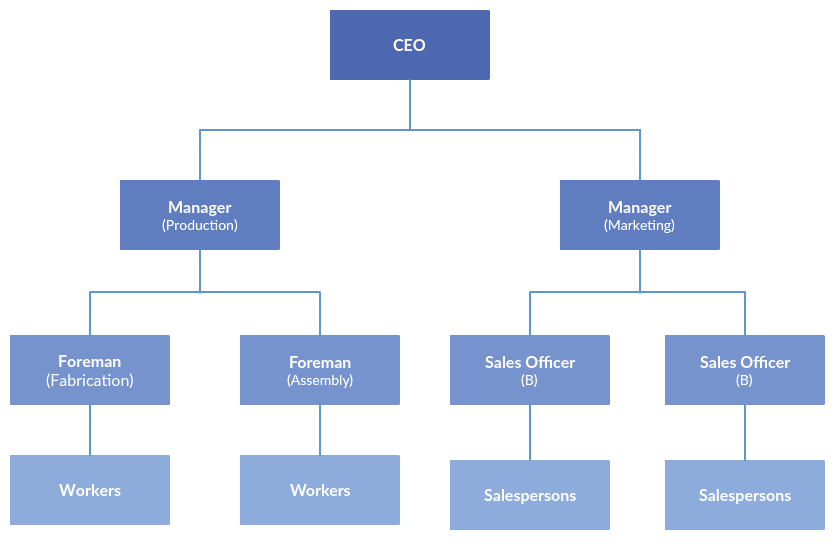
\includegraphics[scale=0.4]{gambar/organization-structure.png}
  % Keterangan gambar yang diinputkan
  \caption{Struktur organisasi PT. NASA}
  % Label referensi dari gambar yang diinputkan
  \label{fig:OrganizationStructure}
\end{figure}

% Contoh penggunaan referensi dari gambar yang diinputkan
Seperti yang bisa dilihat pada Gambar \ref{fig:OrganizationStructure}, \lipsum[15]

  \cleardoublepage

  % Bab 3 tunjauan pustaka
  % Ubah kalimat sesuai dengan judul dari bab ini
\chapter{TINJAUAN PUSTAKA}

% Ubah konten-konten berikut sesuai dengan yang ingin diisi pada bab ini

\section{Roket Luar Angkasa}

% Contoh input gambar dengan format *.jpg
\begin{figure} [ht] \centering
  % Nama dari file gambar yang diinputkan
  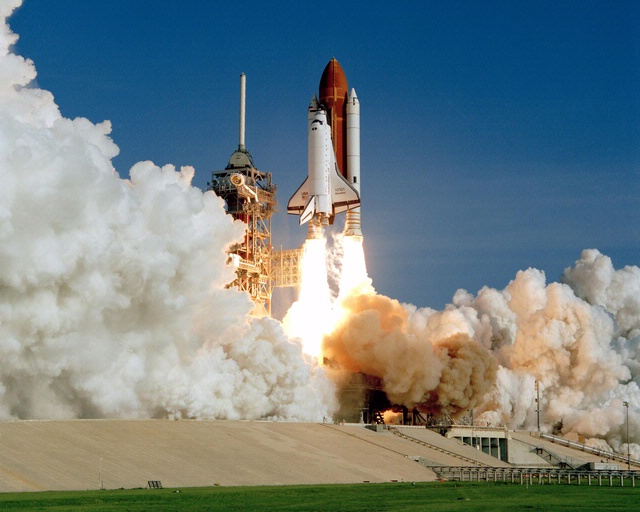
\includegraphics[scale=0.3]{gambar/space-shuttle.jpg}
  % Keterangan gambar yang diinputkan
  \caption{Peluncuran pesawat luar angkasa Discovery \citep{DiscoverySpaceShuttle}}
  % Label referensi dari gambar yang diinputkan
  \label{fig:SpaceShuttle}
\end{figure}

Roket luar angkasa merupakan \lipsum[16][1-10]

% Contoh penggunaan referensi dari gambar yang diinputkan
\emph{Discovery}, Gambar \ref{fig:SpaceShuttle}, merupakan \lipsum[17][1-9]

\section{Gravitasi}

Gravitasi merupakan \lipsum[18][1-10]

\subsection{Hukum Newton}

% Contoh penggunaan referensi dari pustaka
Newton \citep{Newton1687} pernah merumuskan bahwa \lipsum[19]
% Contoh penggunaan referensi dari persamaan
Kemudian menjadi persamaan seperti pada persamaan \ref{eq:FirstNewtonLaw}.

% Contoh pembuatan persamaan
\begin{equation}
  % Label referensi dari persamaan yang dibuat
  \label{eq:FirstNewtonLaw}
  % Baris kode persamaan yang dibuat
  \sum \mathbf{F} = 0\; \Leftrightarrow\; \frac{\mathrm{d} \mathbf{v} }{\mathrm{d}t} = 0.
\end{equation}

\subsection{Anti Gravitasi}

Anti gravitasi merupakan \lipsum[20]

  \cleardoublepage

  % Bab 4 desain dan implementasi
  % Ubah kalimat sesuai dengan judul dari bab ini
\chapter{DESAIN DAN IMPLEMENTASI}

% Ubah konten-konten berikut sesuai dengan yang ingin diisi pada bab ini

\section{Deskripsi Sistem}

Sistem akan dibuat dengan \lipsum[21][1-12]

\section{Implementasi Alat}

Alat diimplementasikan dengan \lipsum[22]

% Contoh pembuatan code snippet
\begin{lstlisting}[
  language=C++,
  label={lst:Hello World},
  caption={Program hello world}
]
#include <iostream>

int main() {
    std::cout << "Hello World!";
    return 0;
}
\end{lstlisting}

% Contoh penggunaan referensi dari code snippet yang diinputkan
Seperti contoh pada baris program Listing \ref{lst:Hello World} dan Listing \ref{lst:PrimeNumber}, \lipsum[23]

% Contoh input code snippet
\lstinputlisting[
  % Bahasa yang digunakan oleh code snippet
  language=Python,
  % Label referensi dari code snippet yang diinputkan
  label={lst:PrimeNumber},
  % Keterangan dari code snippet yang diinputkan
  caption={Program perhitungan bilangan prima}
% Nama dari file code snippet yang diinputkan
]{program/prime-number.py}

  \cleardoublepage

  % Bab 5 pengujian dan evaluasi
  % Ubah kalimat sesuai dengan judul dari bab ini
\chapter{PENGUJIAN DAN EVALUASI}

% Ubah konten-konten berikut sesuai dengan yang ingin diisi pada bab ini

\section{Skenario Pengujian}

Pengujian dilakukan dengan \lipsum[24]

\section{Evaluasi Pengujian}

Dari pengujian yang \lipsum[25][1-10]

% Contoh input konten dari file terpisah
% Contoh pembuatan tabel
\begin{longtable}{|l|l|l|}
  % Keterangan dari tabel yang dibuat
  \caption{Hasil Pengukuran Energi dan Kecepatan}
  % Label referensi dari tabel yang dibuat
  \label{tb:EnergiKecepatan}\\
  % Isi dari tabel yang dibuat
  \hline
  \rowcolor[HTML]{C0C0C0}
  \textbf{Energi} & \textbf{Jarak Tempuh} & \textbf{Kecepatan} \\ \hline
  10 J & 1000 M & 200 M/s \\ \hline
  20 J & 2000 M & 400 M/s \\ \hline
  30 J & 4000 M & 800 M/s \\ \hline
  40 J & 8000 M & 1600 M/s \\ \hline
\end{longtable}


% Contoh penggunaan referensi dari tabel yang dibuat
Sesuai dengan hasil pada Tabel \ref{tb:EnergiKecepatan}, didapatkan bahwa energi yang \lipsum[26]

  \cleardoublepage

  % Bab 6 kesimpulan dan saran
  % Ubah kalimat sesuai dengan judul dari bab ini
\chapter{KESIMPULAN DAN SARAN}

% Ubah konten-konten berikut sesuai dengan yang ingin diisi pada bab ini

\section{Kesimpulan}

Kesimpulan yang kami peroleh dari \lipsum[28][1-3] adalah:

\begin{enumerate}[nolistsep]

  \item Pembuatan \lipsum[29][1-3]

  \item \lipsum[29][4-6]

  \item \lipsum[29][7-9]

\end{enumerate}

\section{Saran}

Saran yang kami ajukan dalam \lipsum[30][1-2] antara lain:

\begin{enumerate}[nolistsep]

  \item Sebaiknya \lipsum[31][1-3]

  \item \lipsum[31][4-6]

  \item \lipsum[31][7-9]

\end{enumerate}

  \cleardoublepage

  % Daftar pustaka
  \renewcommand\bibname{DAFTAR PUSTAKA}
  \addcontentsline{toc}{chapter}{\bibname}
  \bibliographystyle{unsrtnat}
  \bibliography{pustaka/pustaka.bib}
  \cleardoublepage

  % Biografi penulis
  \begin{center}
  \Large\textbf{BIOGRAFI PENULIS}
\end{center}
\vspace{2ex}

\addcontentsline{toc}{chapter}{BIOGRAFI PENULIS}

\begin{wrapfigure}{L}{0.3\textwidth}
  \centering
  \vspace{-3ex}
  % Ubah nama file gambar berikut dengan nama file foto dari mahasiswa pertama
  
\includegraphics[width=0.3\textwidth]{gambar/elon.jpg}
  \vspace{-4ex}
\end{wrapfigure}

% Ubah kalimat berikut dengan biografi dari mahasiswa pertama
\noindent Elon Reeve Musk, lahir pada \lipsum[1]

\vspace{2ex}

\begin{wrapfigure}{L}{0.3\textwidth}
  \centering
  \vspace{-3ex}
  % Ubah nama file gambar berikut dengan nama file foto dari mahasiswa kedua
  
\includegraphics[width=0.3\textwidth]{gambar/felix.jpg}
  \vspace{-4ex}
\end{wrapfigure}

% Ubah kalimat berikut dengan biografi dari mahasiswa kedua
\noindent Felix Arvid Ulf Kjellberg, lahir pada \lipsum[2]

  \cleardoublepage

\end{document}
